\section{Hardware Constraints in the 1980s}
In the 1980s, game consoles and home computers faced severe hardware limitations. Storage media, such as ROM cartridges or tapes were measured in kilobytes, not megabytes. Processing power was also extremely low: CPUs were only 4‑bit or 8‑bit and lacked hardware multipliers. So they could not perform complex floating‑point calculations.

\begin{figure}[h]
\centering
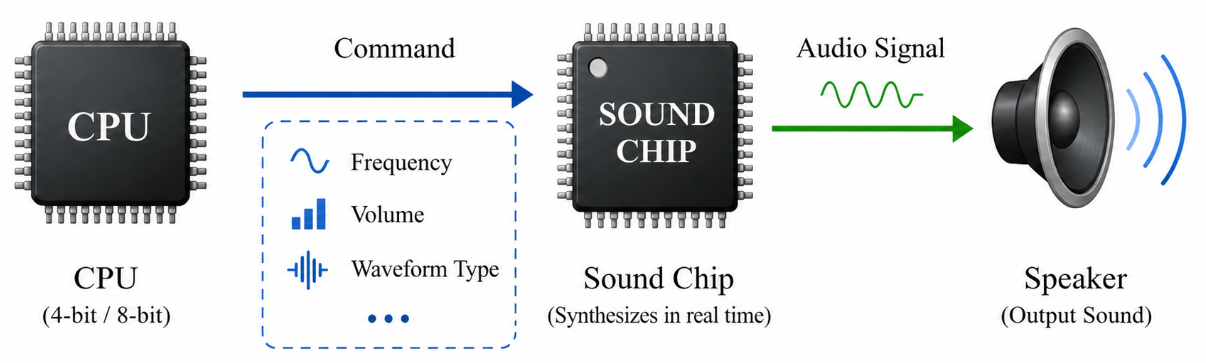
\includegraphics[width=0.65\linewidth]{pictures/command-driven.png}
\caption{Block diagram of command‑driven audio: CPU $\to$ Commands $\to$ Sound Chip $\to$ Speaker.}
\label{fig:command-driven}
\end{figure}

To work within these constraints, engineers invented command‑driven audio (Figure ~\ref{fig:command-driven}). Instead of streaming heavy audio data, the CPU sent simple commands (frequency, volume, waveform type) to a dedicated sound chip, which synthesized the sound in real time. This saved precious storage and CPU cycles.

